\documentclass[tikz]{standalone}

\usetikzlibrary{positioning}

\begin{document}
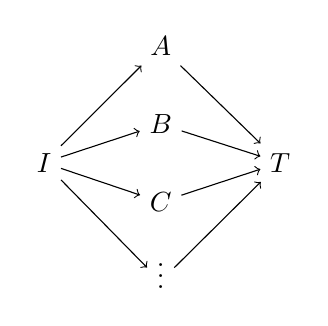
\begin{tikzpicture}
	\node (A) {$A$};
	\node [below=0.5cm of A] (B) {$B$};
	\node [below=0.5cm of B] (C) {$C$};
	\node [below=0.2cm of C] (D) {$\vdots$};
	\node [below left =0.0cm and 1.0cm of B] (I) {$I$};
	\node [below right=0.0cm and 1.0cm of B] (T) {$T$};
	\draw [->] (I) to (A);
	\draw [->] (I) to (B);
	\draw [->] (I) to (C);
	\draw [->] (I) to (D.west);
	\draw [->] (A) to (T);
	\draw [->] (B) to (T);
	\draw [->] (C) to (T);
	\draw [->] (D.east) to (T);
\end{tikzpicture}
\end{document}
